% Chapter Template

\chapter{Evaluation of VAD algorithms} % Main chapter title

\label{Chapter4} % Change X to a consecutive number; for referencing this chapter elsewhere, use \ref{ChapterX}

\lhead{Chapter 4. \emph{Evaluation of VAD algorithms}} % Change X to a consecutive number; this is for the header on each page - perhaps a shortened title

%------------------------------------------------
%	SECTION 1
%------------------------------------------------

\section{Main Section 1}

%------------------------------------------------
%	SECTION 1
%------------------------------------------------

\section{Main Section 2}

\begin{figure}[htbp]
	\centering
		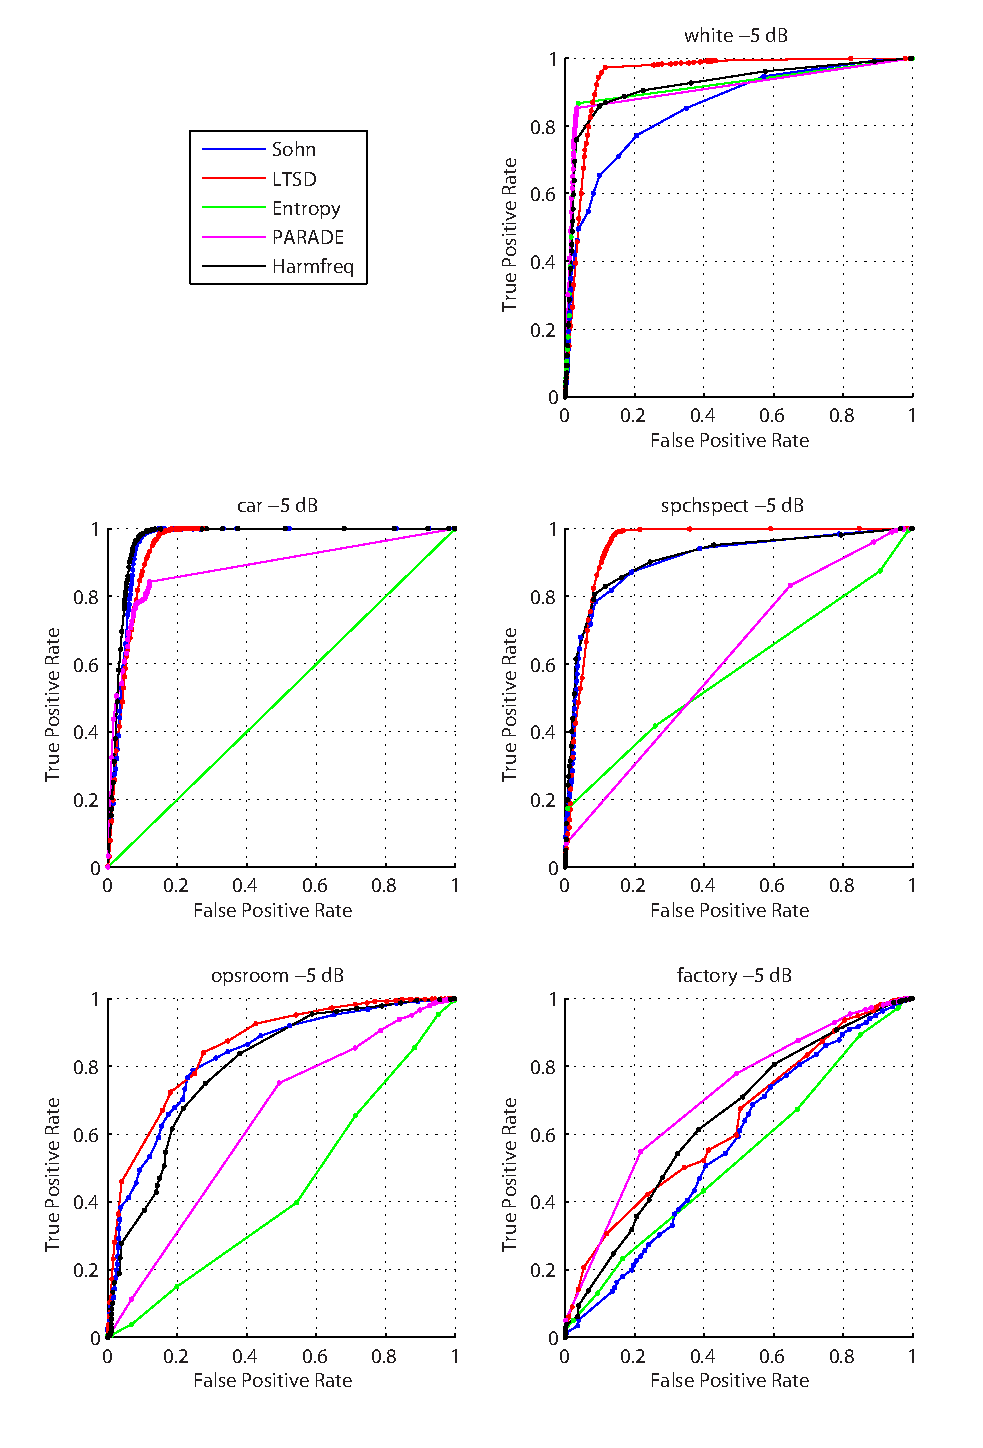
\includegraphics[width=1.0\columnwidth]{Figures/Chapter3/-5dBh.pdf}
		\rule{37em}{0.5pt}
	\caption[ROC curves of the evaluated algorithms \emph{with} hang-over under -5 dB SNR]{ROC curves of the evaluated VAD algorithms \emph{with} hang-over under -5 dB SNR}
	\label{fig:-5dBh}
\end{figure}

\begin{table}[htbp]
\center
\begin{tabular}{c|c|c|c|c|c!{\vrule width 1.5pt}c|}
\cline{2-7}
 & white & car & spchspect & opsroom & factory & average \\ \hline
\multicolumn{1}{ |c| }{Sohn} & 0.8561 & 0.9595 & 0.9063 & 0.8276 & 0.5671 & 0.8233\\ \hline
\multicolumn{1}{ |c| }{LTSD} & \textcolor{LimeGreen}{0.9497} & 0.9496 & \textcolor{LimeGreen}{0.9502} & \textcolor{LimeGreen}{0.8586} & 0.6345 & \textcolor{LimeGreen}{\textbf{0.8685}}\\ \hline
\multicolumn{1}{ |c| }{Entropy} & 0.9160 & \textcolor{red}{0.4999} & \textcolor{red}{0.5807} & \textcolor{red}{0.4350} & \textcolor{red}{0.5315} & \textcolor{red}{\textbf{0.5926}}\\ \hline
\multicolumn{1}{ |c| }{PARADE} & \textcolor{red}{0.9117} & 0.8853 & 0.6159 & 0.6339 & \textcolor{LimeGreen}{0.7071} & 0.7508\\ \hline
\multicolumn{1}{ |c| }{Harmfreq} & 0.9209 & \textcolor{LimeGreen}{0.9676} & 0.9126 & 0.7992 & 0.6425 & 0.8486\\ \hline
\end{tabular}
\caption[AUC values of the evaluated algorithms \emph{with} hang-over under -5 dB SNR]{AUC values of the evaluated VAD algorithms \emph{with} hang-over under -5 dB SNR}
\label{tab:AUC-5dBh}
\end{table}

\begin{figure}[htbp]
	\centering
		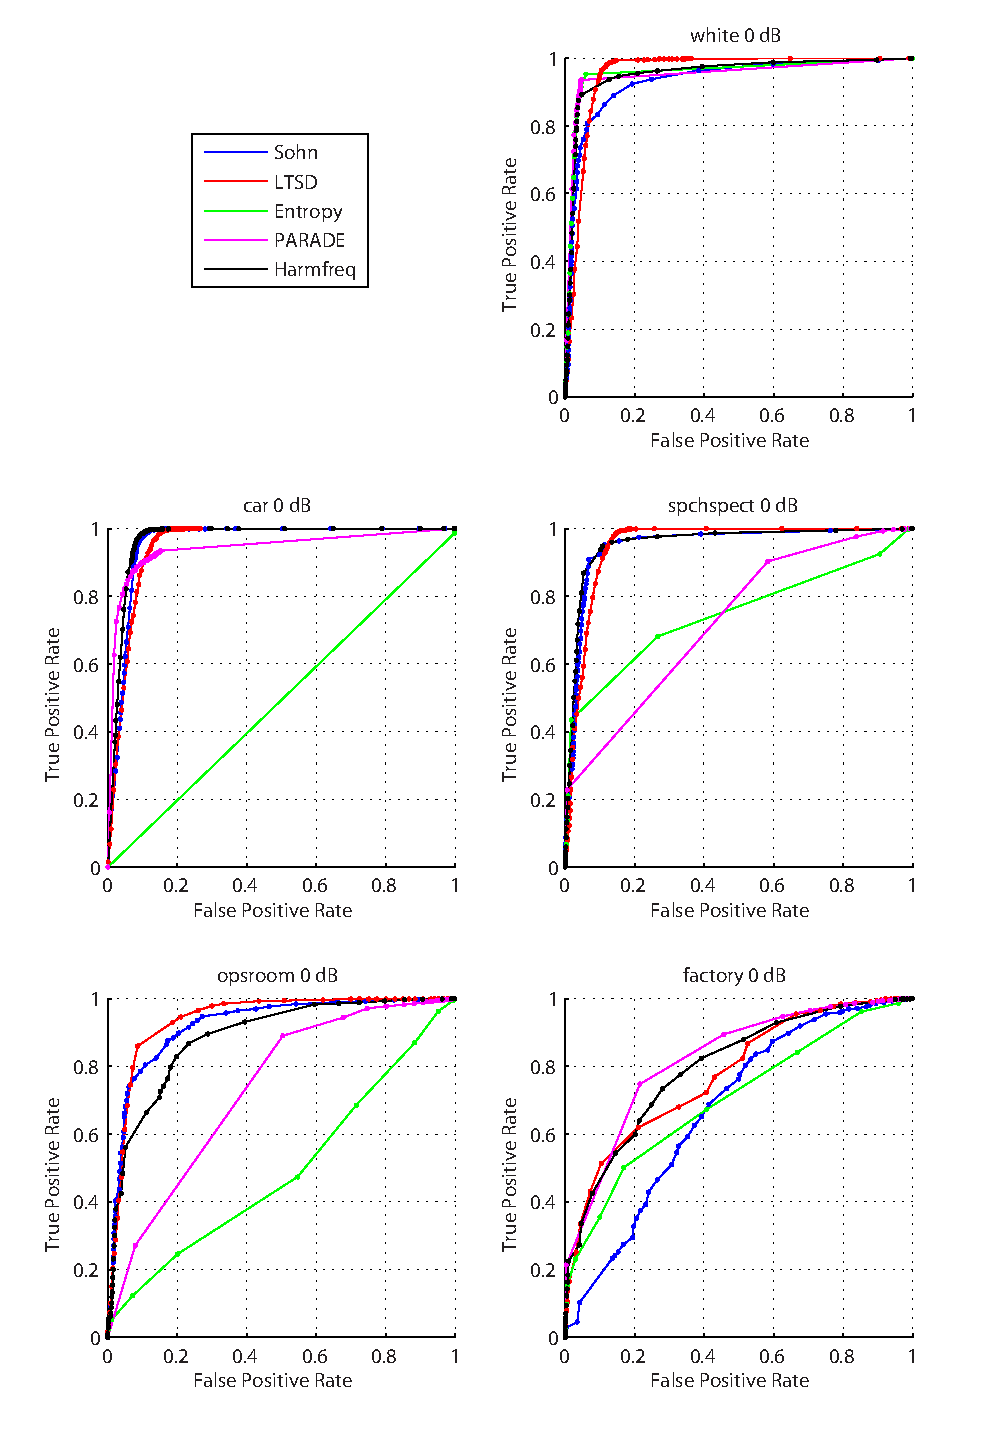
\includegraphics[width=1.0\columnwidth]{Figures/Chapter3/0dBh.pdf}
		\rule{37em}{0.5pt}
	\caption[ROC curves of the evaluated algorithms \emph{with} hang-over under 0 dB SNR]{ROC curves of the evaluated VAD algorithms \emph{with} hang-over under 0 dB SNR}
	\label{fig:0dBh}
\end{figure}

\begin{table}[htbp]
\center
\begin{tabular}{c|c|c|c|c|c!{\vrule width 1.5pt}c|}
\cline{2-7}
 & white & car & spchspect & opsroom & factory & average \\ \hline
\multicolumn{1}{ |c| }{Sohn} & \textcolor{red}{0.9334} & 0.9573 & 0.9506 & 0.9226 & \textcolor{red}{0.6740} & 0.8876\\ \hline
\multicolumn{1}{ |c| }{LTSD} & 0.9555 & 0.9498 & \textcolor{LimeGreen}{0.9508} & \textcolor{LimeGreen}{0.9390} & 0.7770 & \textcolor{LimeGreen}{\textbf{0.9144}}\\ \hline
\multicolumn{1}{ |c| }{Entropy} & \textcolor{LimeGreen}{0.9564} & \textcolor{red}{0.4942} & 0.7466 & \textcolor{red}{0.4926} & 0.7030 & \textcolor{red}{\textbf{0.6785}}\\ \hline
\multicolumn{1}{ |c| }{PARADE} & 0.9513 & 0.9415 & \textcolor{red}{0.7267} & 0.7329 & \textcolor{LimeGreen}{0.8225} & 0.8350\\ \hline
\multicolumn{1}{ |c| }{Harmfreq} & 0.9541 & \textcolor{LimeGreen}{0.9673} & 0.9557 & 0.8862 & 0.7976 & 0.9122\\ \hline
\end{tabular}
\caption[AUC values of the evaluated algorithms \emph{with} hang-over under 0 dB SNR]{AUC values of the evaluated VAD algorithms \emph{with} hang-over under 0 dB SNR}
\label{tab:AUC0dBh}
\end{table}

\begin{figure}[htbp]
	\centering
		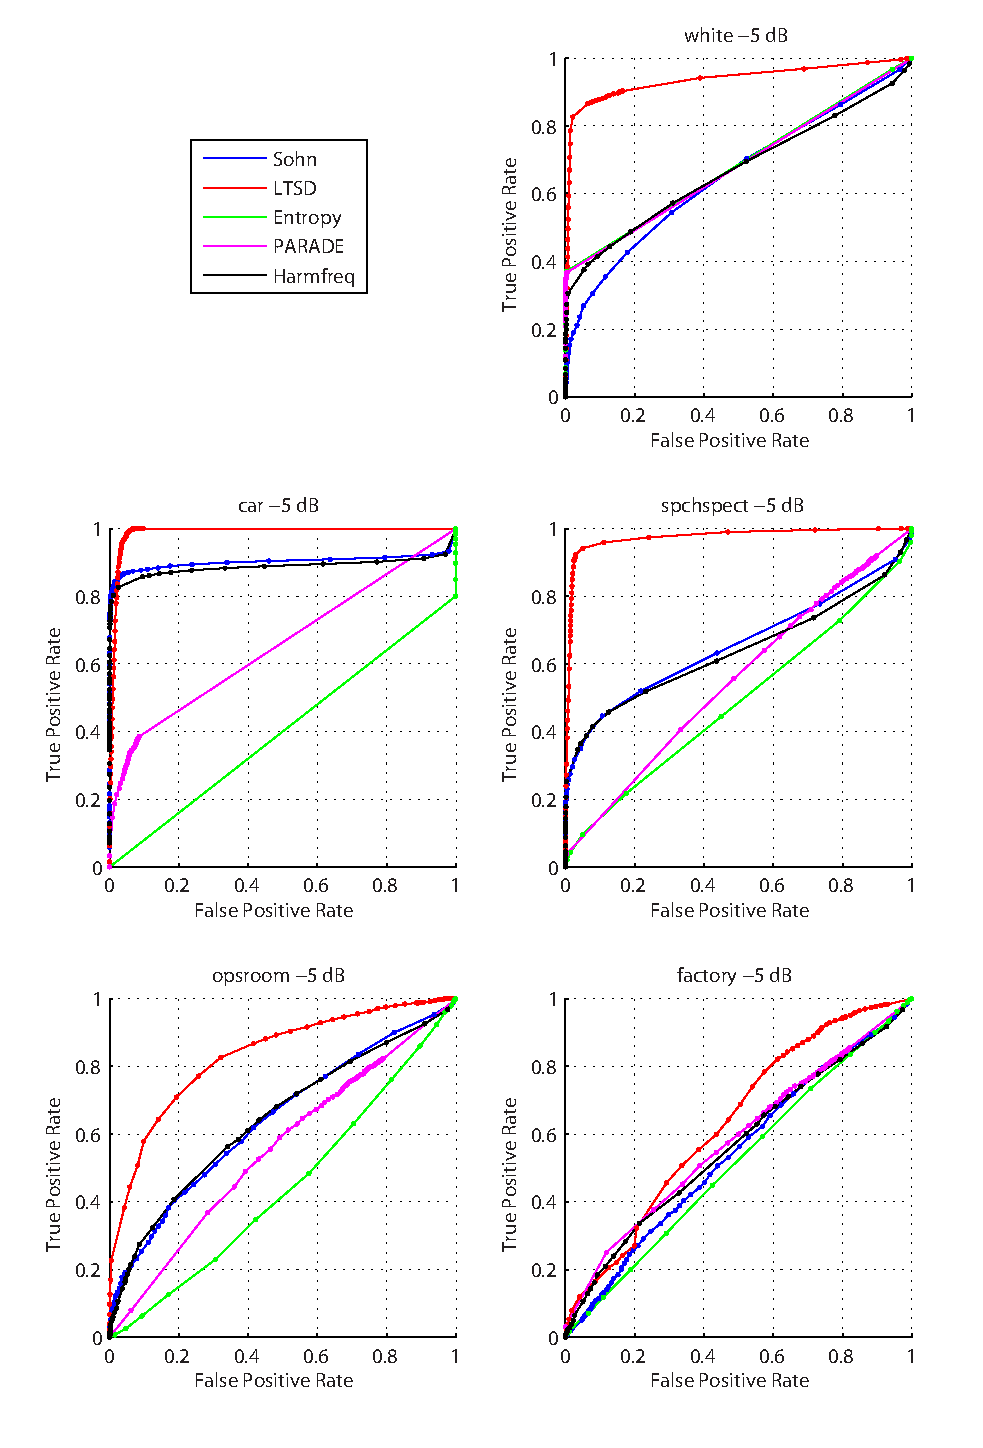
\includegraphics[width=1.0\columnwidth]{Figures/Chapter3/-5dBnoh.pdf}
		\rule{37em}{0.5pt}
	\caption[ROC curves of the evaluated algorithms \emph{without} hang-over under -5 dB SNR]{ROC curves of the evaluated VAD algorithms \emph{without} hang-over under -5 dB SNR}
	\label{fig:-5dBnoh}
\end{figure}

\begin{figure}[htbp]
	\centering
		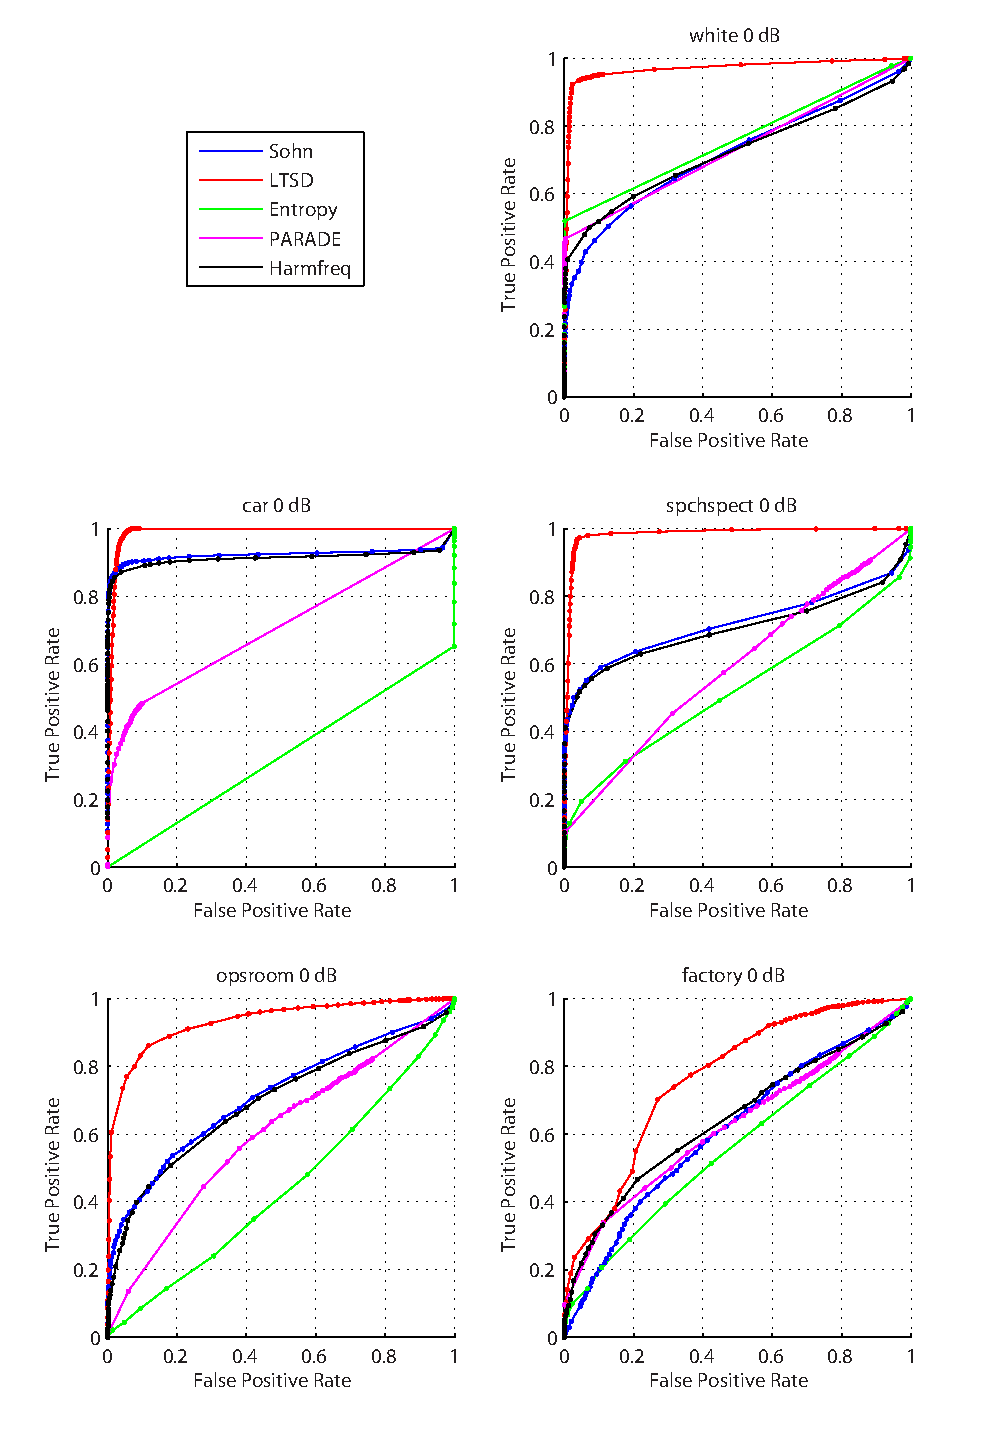
\includegraphics[width=1.0\columnwidth]{Figures/Chapter3/0dBnoh.pdf}
		\rule{37em}{0.5pt}
	\caption[ROC curves of the evaluated algorithms \emph{without} hang-over under 0 dB SNR]{ROC curves of the evaluated VAD algorithms \emph{without} hang-over under 0 dB SNR}
	\label{fig:0dBnoh}
\end{figure}